\documentclass[tikz,border=10pt]{standalone}
\usepackage{mathabx}
\usepackage{stackengine}
\usetikzlibrary{backgrounds}
\usepackage{newunicodechar}
\newunicodechar{♮}{$\natural$}
\newunicodechar{♭}{$\flat$}
\newunicodechar{♯}{$\sharp$}
\newunicodechar{➚}{$\nearrow$}
\newunicodechar{➘}{$\searrow$}
\newunicodechar{ʼ}{'}
\newunicodechar{Ȧ}{\stackon[0.8pt]{A}{.}}
\newunicodechar{Ḃ}{\stackon[0.8pt]{B}{.}}
\newunicodechar{Ċ}{\stackon[0.8pt]{C}{.}}
\newunicodechar{Ḋ}{\stackon[0.8pt]{D}{.}}
\newunicodechar{Ė}{\stackon[0.8pt]{E}{.}}
\newunicodechar{Ḟ}{\stackon[0.8pt]{F}{.}}
\newunicodechar{Ġ}{\stackon[0.8pt]{G}{.}}


\def\centerarc[#1](#2)(#3:#4:#5);%
{
  \draw[#1]([shift=(#3:#5)]#2) arc (#3:#4:#5);
}


\begin{document}
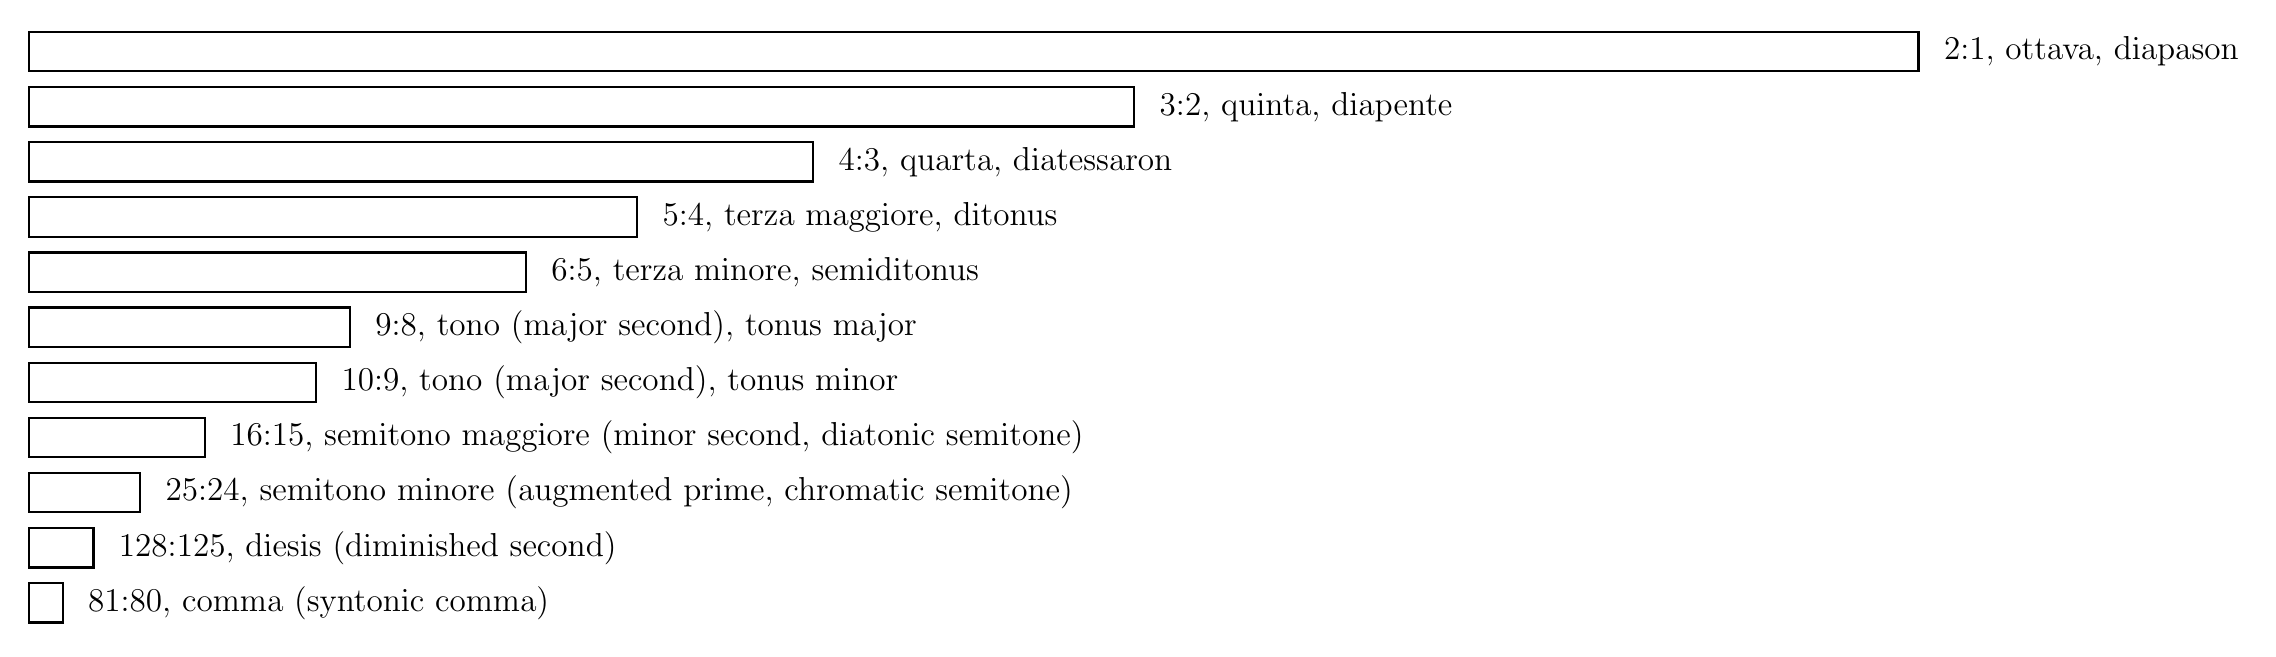
\begin{tikzpicture}

\draw[thick] (0.0, -0.25) -- (0.43011245, -0.25) -- (0.43011245, 0.25) -- (0.0, 0.25) --  cycle;
\node[anchor=west] at (0.63011247, 0.0) { \large 81:80, comma (syntonic comma) };
\draw[thick] (0.0, 0.45000002) -- (0.82115173, 0.45000002) -- (0.82115173, 0.95) -- (0.0, 0.95) --  cycle;
\node[anchor=west] at (1.0211518, 0.7) { \large 128:125, diesis (diminished second) };
\draw[thick] (0.0, 1.15) -- (1.4134048, 1.15) -- (1.4134048, 1.65) -- (0.0, 1.65) --  cycle;
\node[anchor=west] at (1.6134049, 1.4) { \large 25:24, semitono minore (augmented prime, chromatic semitone) };
\draw[thick] (0.0, 1.85) -- (2.2345567, 1.85) -- (2.2345567, 2.3500001) -- (0.0, 2.3500001) --  cycle;
\node[anchor=west] at (2.4345567, 2.1000001) { \large 16:15, semitono maggiore (minor second, diatonic semitone) };
\draw[thick] (0.0, 2.55) -- (3.6479611, 2.55) -- (3.6479611, 3.05) -- (0.0, 3.05) --  cycle;
\node[anchor=west] at (3.8479612, 2.8) { \large 10:9, tono (major second), tonus minor };
\draw[thick] (0.0, 3.25) -- (4.078074, 3.25) -- (4.078074, 3.75) -- (0.0, 3.75) --  cycle;
\node[anchor=west] at (4.278074, 3.5) { \large 9:8, tono (major second), tonus major };
\draw[thick] (0.0, 3.95) -- (6.312631, 3.95) -- (6.312631, 4.4500003) -- (0.0, 4.4500003) --  cycle;
\node[anchor=west] at (6.5126314, 4.2000003) { \large 6:5, terza minore, semiditonus };
\draw[thick] (0.0, 4.65) -- (7.7260346, 4.65) -- (7.7260346, 5.15) -- (0.0, 5.15) --  cycle;
\node[anchor=west] at (7.9260345, 4.9) { \large 5:4, terza maggiore, ditonus };
\draw[thick] (0.0, 5.35) -- (9.960592, 5.35) -- (9.960592, 5.85) -- (0.0, 5.85) --  cycle;
\node[anchor=west] at (10.160592, 5.6) { \large 4:3, quarta, diatessaron };
\draw[thick] (0.0, 6.05) -- (14.038665, 6.05) -- (14.038665, 6.55) -- (0.0, 6.55) --  cycle;
\node[anchor=west] at (14.238665, 6.3) { \large 3:2, quinta, diapente };
\draw[thick] (0.0, 6.75) -- (23.999256, 6.75) -- (23.999256, 7.25) -- (0.0, 7.25) --  cycle;
\node[anchor=west] at (24.199255, 7.0) { \large 2:1, ottava, diapason };
\end{tikzpicture}
\end{document}